\documentclass[11pt]{amsart}
\usepackage{geometry}                % See geometry.pdf to learn the layout options. There are lots.
\geometry{letterpaper}                   % ... or a4paper or a5paper or ... 
%\geometry{landscape}                % Activate for for rotated page geometry
%\usepackage[parfill]{parskip}    % Activate to begin paragraphs with an empty line rather than an indent
\usepackage{graphicx}
\usepackage{amssymb}
\usepackage{epstopdf}
\DeclareGraphicsRule{.tif}{png}{.png}{`convert #1 `dirname #1`/`basename #1 .tif`.png}

\title{Supervised ML: Classification, Final Project}
\author{Jackson Walters}
\date{}                                           % Activate to display a given date or no date

\begin{document}
\maketitle
%\section{}
%\subsection{}

\section{Introduction}

This project is for the Exploratory Data Analysis for Machine Learning certification from IBM via Coursera. The long-term goal is to create a t-SNE plot to observe clustering of mental health disorders based on symptom data, as in the linked paper\footnote{https://www.ncbi.nlm.nih.gov/pmc/articles/PMC6783390/}. I would like to include additional data based on life factors such as income, housing status, and insurance status. The idea is that if someone has no income, is unhoused, and uninsured then they would be much more likely to be classified as having a mental illness. I want to go beyond correlation, and see clustering. \\


\section{PCA and t-SNE for MNIST sample data}

For now, I implemented code from here \footnote{https://medium.com/@violante.andre/an-introduction-to-t-sne-with-python-example-47e6ae7dc58f}, and removed the SAS connection. I rewrote it in pure Python with sklearn. I did both PCA and t-SNE on the MNIST data, and plots are shown below. \\

All code is publicly available on GitHub \footnote{https://github.com/jacksonwalters/ml-examples}.

\begin{figure}[h]
\caption{PCA plot of MNIST handwritten digits data}
\centering
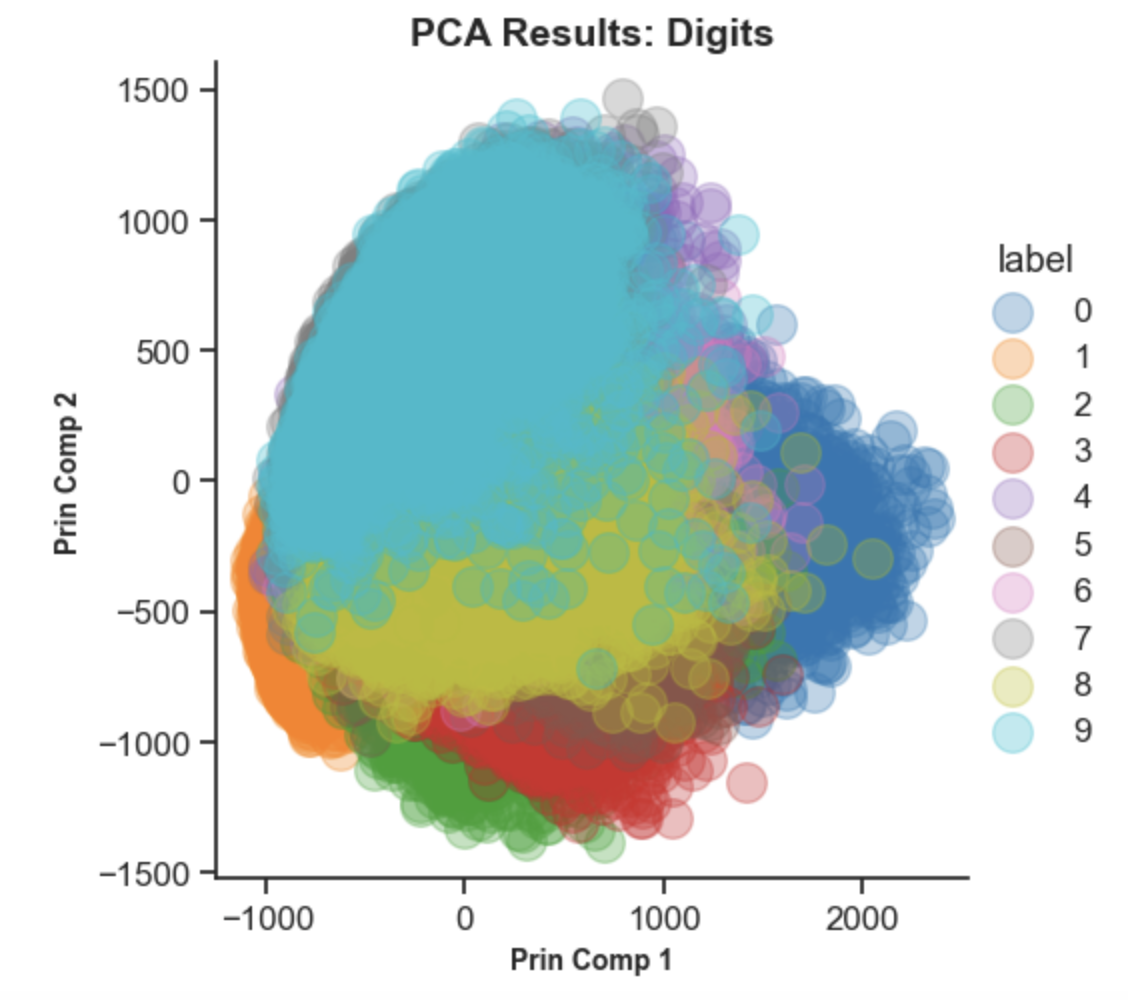
\includegraphics[width=0.5\textwidth]{PCA_plot_MNIST}
\end{figure}

\begin{figure}[h]
\caption{t-SNE plot of MNIST handwritten digits data}
\centering
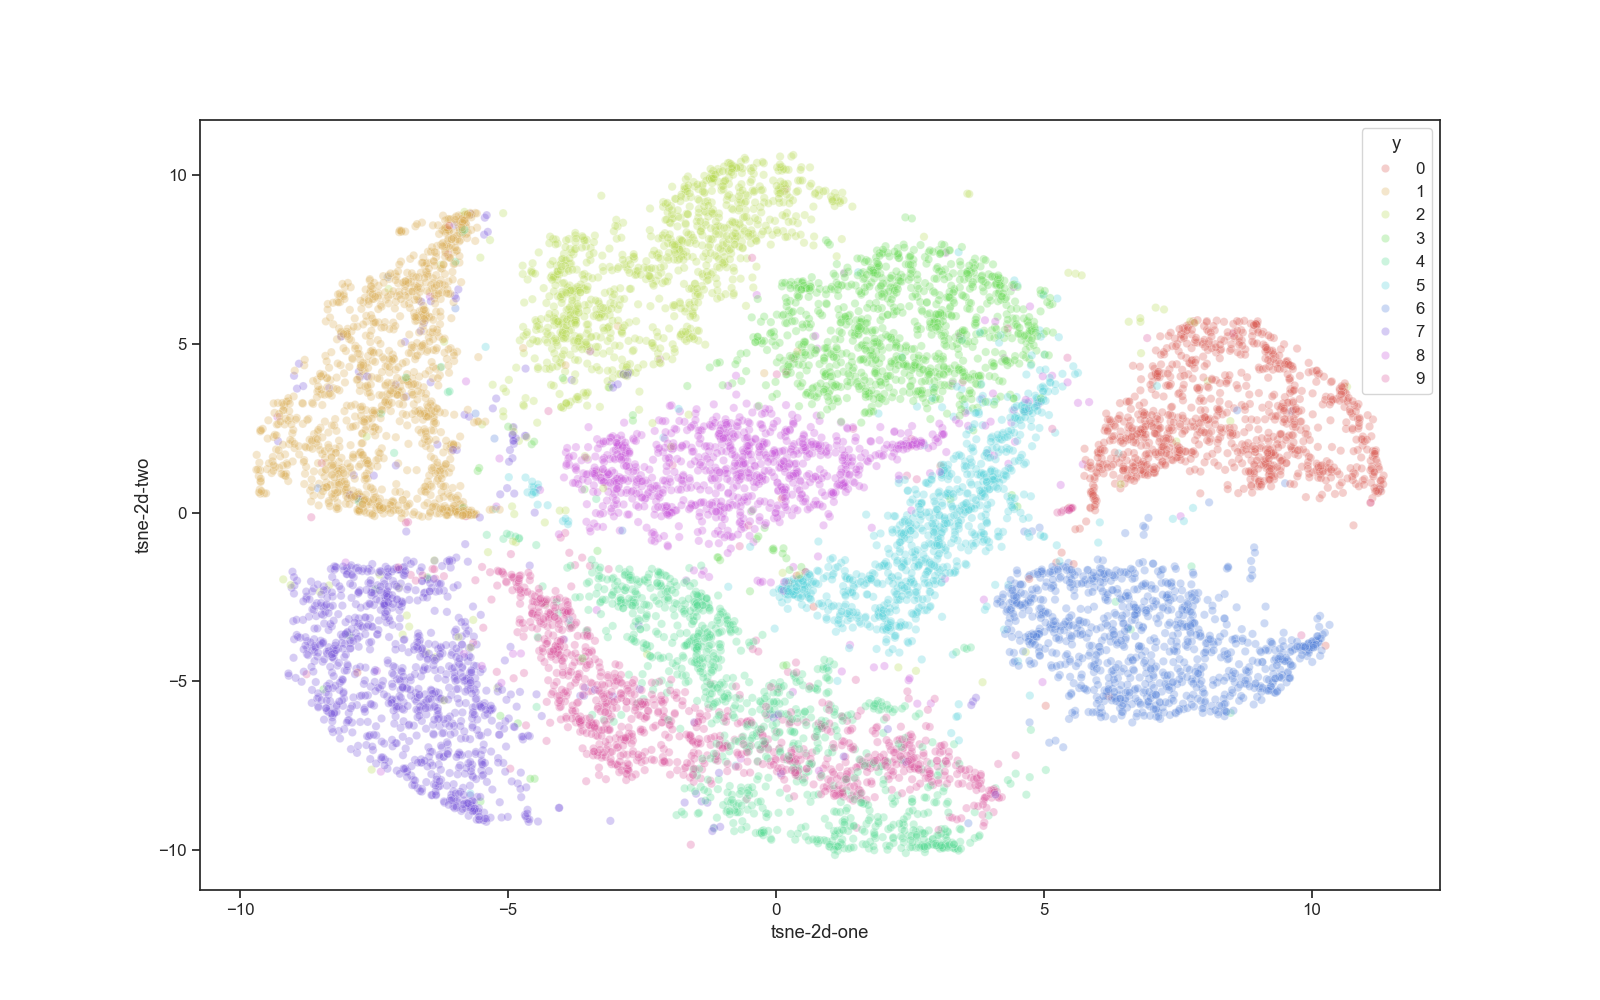
\includegraphics[width=0.5\textwidth]{t-SNE_plot_MNIST}
\end{figure}

\section{Mental Health Client-Level Data}

The data are 6.5mil rows and around 50 columns. There are 13 disorder codes listed, each a binary variable. The rest are life factors including employment, demographics like age, gender, ethnicity, geographic information, and more. I have dropped the irrelevant columns, one-hot encoded the categorical columns, and scaled all columns to be in $[0,1]$.

There are a few different ways to think of the labels, but they are all derived from the 13 binary diagnosis columns. This is an example of a multi-label problem, distinct from a multi-output or multi-class problem, though we may transform it into one of these. For example, in one labeling I bin the disorders as [0 disorders, 1 disorder, >1 disorder] giving 15 labels. Another approach is to use a binary encoding so that each 13-tuple of binaries maps to a unique integer between 0-8191 since $2^{13} = 8192$. One could also count the number of disorders, yielding 13 labels, since the maximum sum is 13. Finally, one could use a more sophisticated approach like k-means, which finds a centroid of clusters and expands outwards. This is what we will typically use to color the t-SNE and PCA plots:

\begin{figure}[h]
\caption{t-SNE plot of mental health data with k-means labeling}
\centering
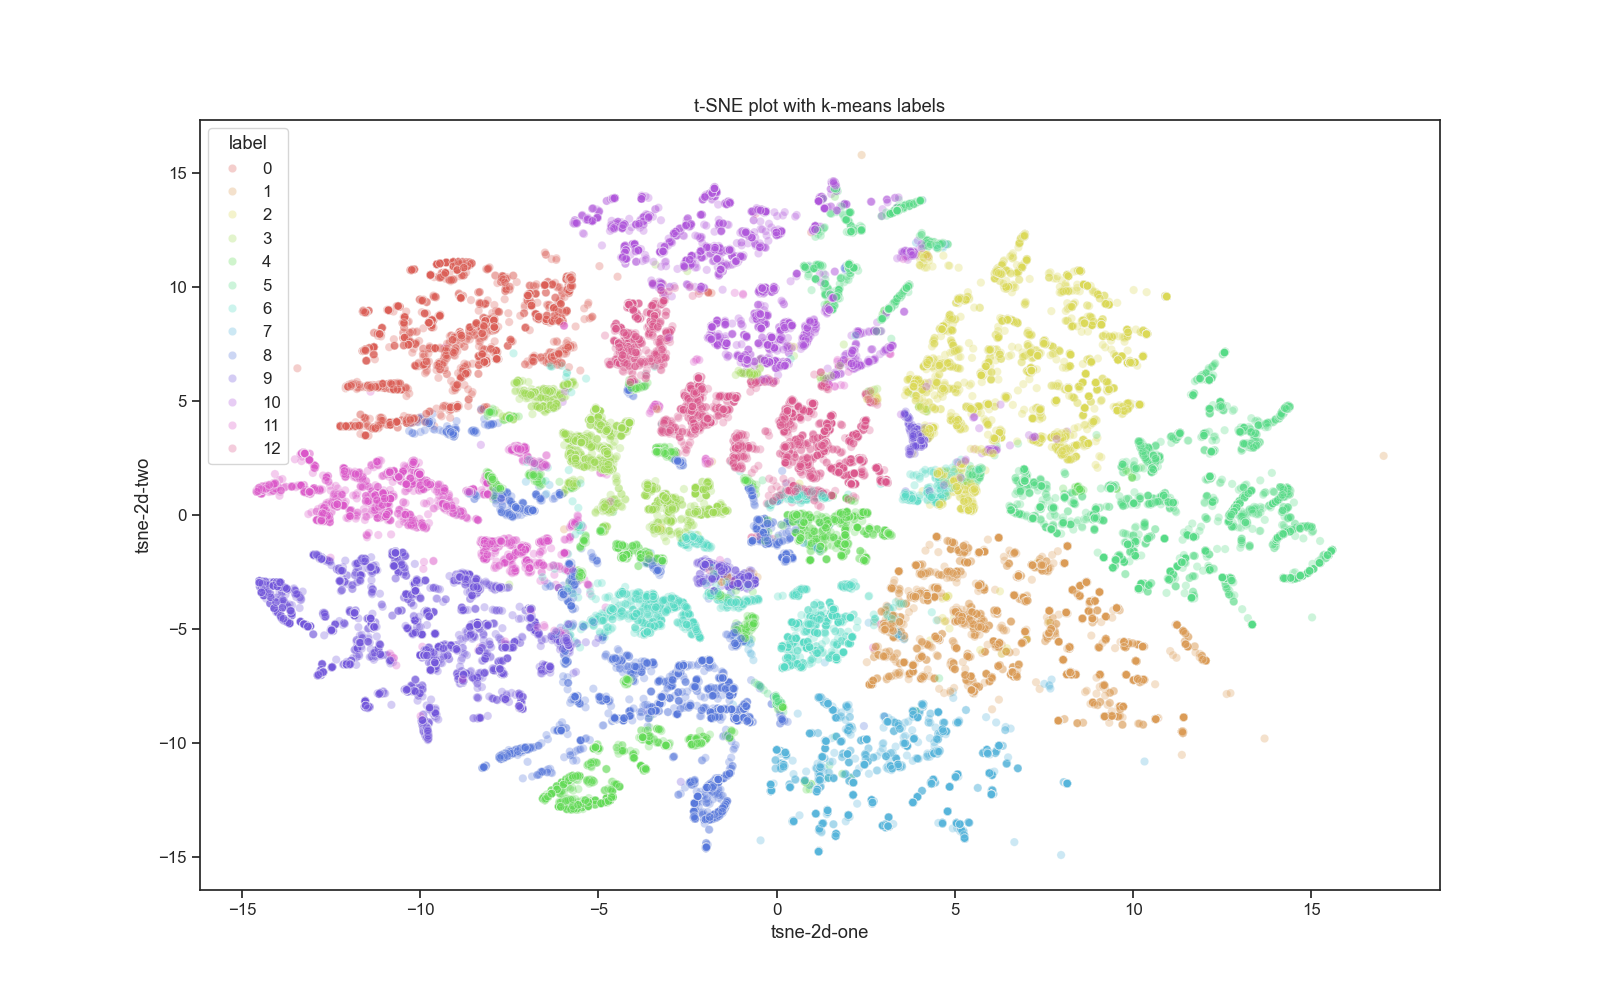
\includegraphics[width=0.5\textwidth]{t-sne_k-means_label.png}
\end{figure}

Here we choose $num_clusters=15$, and we can clearly see some clusters forming, likely from the demographic information but the diagnostic information is included. If we try to label with $unique_disorders$, that is 13 categories for those diagnosed with a unique disorder and two for no disorders and multi-disorder, we obtain the following plot:

\begin{figure}[h]
\caption{t-SNE plot of mental health data with $unique_disorder$ labeling}
\centering
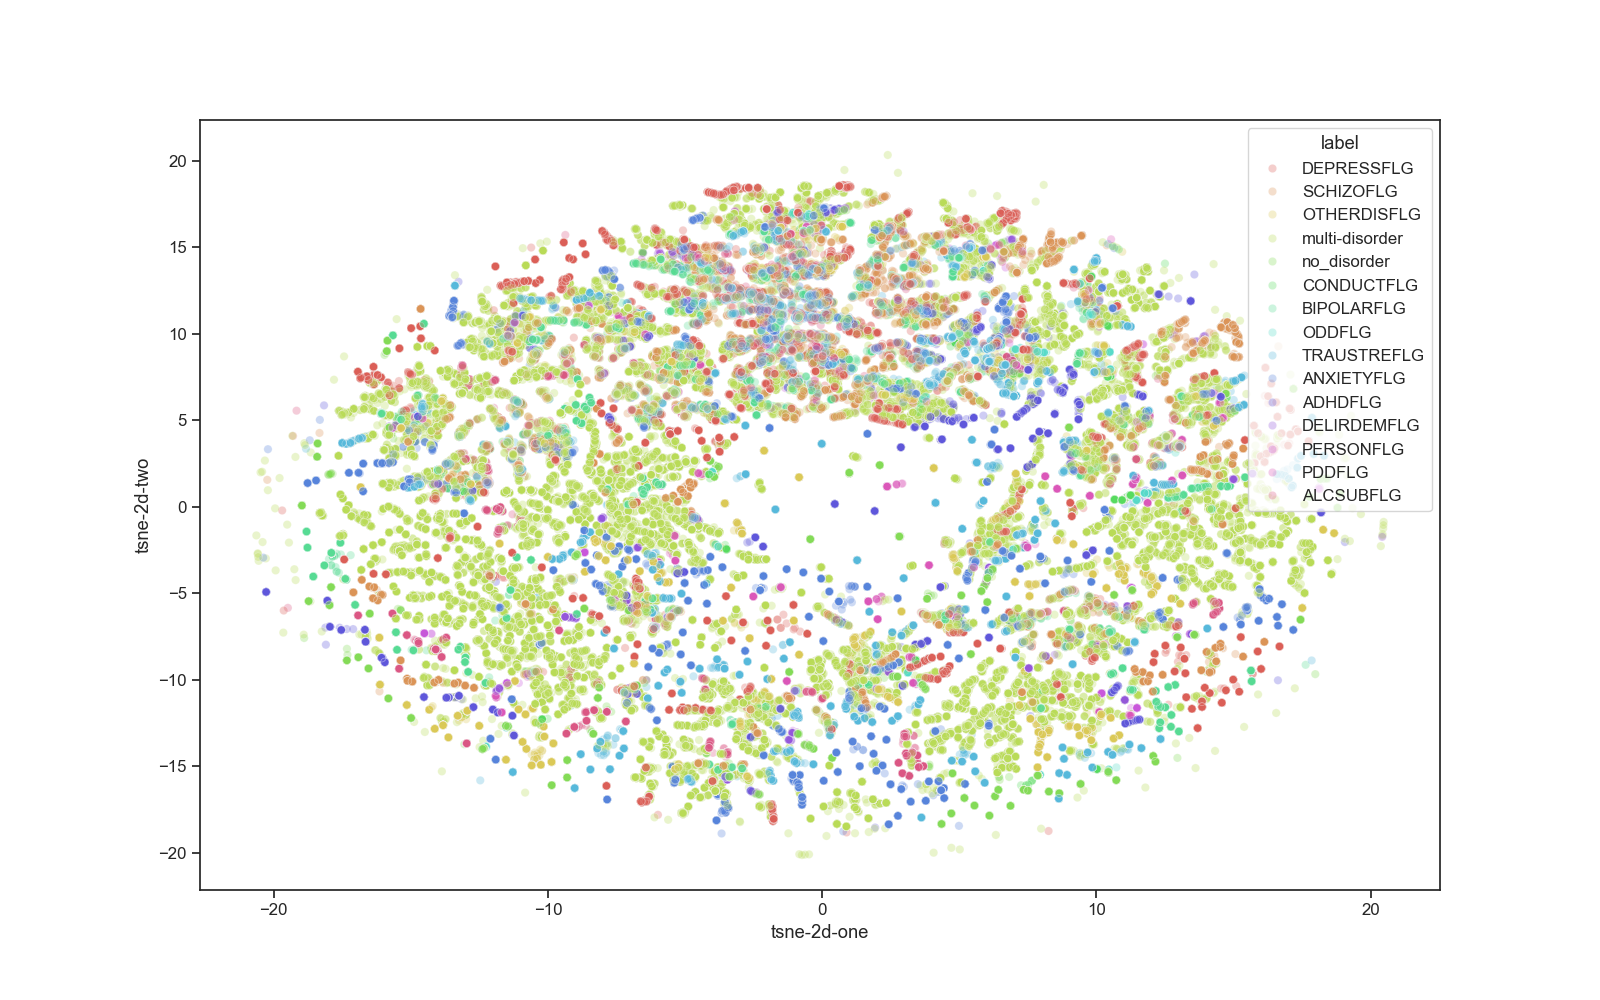
\includegraphics[width=0.5\textwidth]{tsne-plot_unique-disorders_label.png}
\end{figure}

\section{Classification}

We can also attempt the classification problem. That is, given the demographic and life factor data, predict which disorder class the patient falls into. Since we have a number of labelings, we have a number of different problems to consider. 

First we try the unique\_disorders labeling and train a RandomForest classifier. This is a multi-class problem. \\

\noindent accuracy: 0.34965 \\
precision: 0.30545804698445045 \\
recall: 0.34965 \\

Next up we try multi-class LogisticRegression. On the unique\_disorders labeling, performance is similar to RandomForest. However, on the k-means labeling, we achieve much better performance: \\

\noindent accuracy: 0.88315 \\
precision: 0.8819518553140321 \\
recall: 0.88315 \\

This reflects the much better clustering observed with the k-means labeling. Now the demographic and life factors are able to predict which k-means cluster a point will fall into, without diagnostic information. \\

We can try to drop 12/13 disorder columns and just do a logistic regression on the remaining column. This gives 13 separate logistic regressions, one for each disorder. We can then use it as a mutli-label classification, and compute the Hamming loss (a metric for distance between 0/1 datasets). In this case, we obtain hamming\_loss=0.12. \\

Using MultiOutputClassifier or OneVsRestClassifier, we obtain hamming\_loss=.1 in both cases. Using k-nearest-nearbors MLkNN from skmultilearn.adapt, we obtain hamming\_loss=.11. \\

Finally, using MultiOutputClassifier with XGBoost, we obtain hamming\_loss=.1. The accuracy score is modified a bit to "subset", and reads: \\

\noindent accuracy: 17.2\% \\
precision: 46.8\% \\
recall: 19.8\% \\

It's worth noting that just computing the number of multi-labels that are correctly predicted with XGBoost is ~3\%, whereas a random guess would be ~1/8192 = .01\%


\end{document}  